\documentclass[10pt]{article}

\usepackage[margin=1in,top=0.75in]{geometry}
\usepackage{graphicx}
\usepackage{pgfgantt}
\usepackage{float}

\pagenumbering{gobble}
\setlength{\parindent}{0in}

\begin{document}
\begin{center}
	\Large\textbf{Buffalo Byte Swarm: Initial Design Memo}\\[0.1in]
	\large Group 6: Bob French, Dylan Pinos, Zhiyun Yu
\end{center}

\section*{Project Overview}
\subsection*{Problem Definition}
In disaster relief situations (earthquakes, tornadoes, etc.), rescue efforts must first search for people that require assistance before deploying a rescue team to that location. This searching stage consumes critical time in which lives could be saved, and spreads resources thin as a result of having to split resources between searching and rescuing. Our projects aim is not to eliminate the searching step entirely, as the Buffalo Byte has limited resources and could not hope to achieve the same effectiveness, mostly due to the sensor limitations. Our aim is instead, to provide a quick preliminary survey of the area, providing information such as the areas where people in need of rescue are more concentrated, as well as specific locations where people in need of rescue are suspected to be. Although our project cannot be relied on as a standalone system, it will quickly perform preliminary search tasks, freeing up search team resources for more specialized tasks. The Buffalo Byte platform fits our needs well as they are small and do not pose the risk of causing harm accidentally, and they are cheap and easy to mass produce. The latter is especially important as it is inevitable that not all the Buffalo Bytes will be able to be retrieved after they are deployed. If we were to use a more sophisticated platform, this could result in heavy monetary losses but by using the Buffalo Byte, monetary losses will be minimal.
\subsection*{Alternative Solutions}
\underline{RecoNode}\\[0.5\baselineskip]
Our Buffalo Byte mesh network surpasses alternatives by balancing cost, scalability, and rapid deployment. Unlike RecoNode’s complex, custom-built hardware, Buffalo Byte leverages off-the-shelf components, making it faster, cheaper, and easier to implement. Other systems have significant trade-offs: Heterogeneous Robot Teams enable specialized roles but require complex coordination and expensive hardware. Tethered Systems provide reliable power but severely limit mobility. WSAC Networks support distributed control but demand precise synchronization and high computational power. Dual-Baseband Radios enhance network reliability but are difficult to integrate with commercial components. Vision-Based AI aids navigation but is impractical for smaller robots due to high processing needs. RTOS improves responsiveness but adds design complexity. Our tiny, agile Buffalo Byte robots excel in disaster scenarios, navigating tight spaces, quickly forming resilient networks, and working as a swarm. While RecoNode prioritizes high-powered, reconfigurable computing, Buffalo Byte focuses on efficiency, adaptability, and real-world usability, making it the superior choice for search and rescue.
\subsection*{Proposed Approach}
The approach we plan to take is to create a mesh network using a large number of Buffalo Bytes, and a central node/server, hosted on a Raspberry Pi or similar. Our system will be flexible, allowing a dynamic number of Buffalo Bytes to be used, which could be anywhere from tens to multiple hundreds depending on the scale of the use case. The Buffalo Bytes will travel across the affected area and take sensor readings at certain points specified by the main node. If human presence is detected, the Buffalo Byte will send it's location through the mesh network back to the main node to signify that there may be someone in need of rescuing at that location.

\section*{Conceptual Model}
\begin{center}
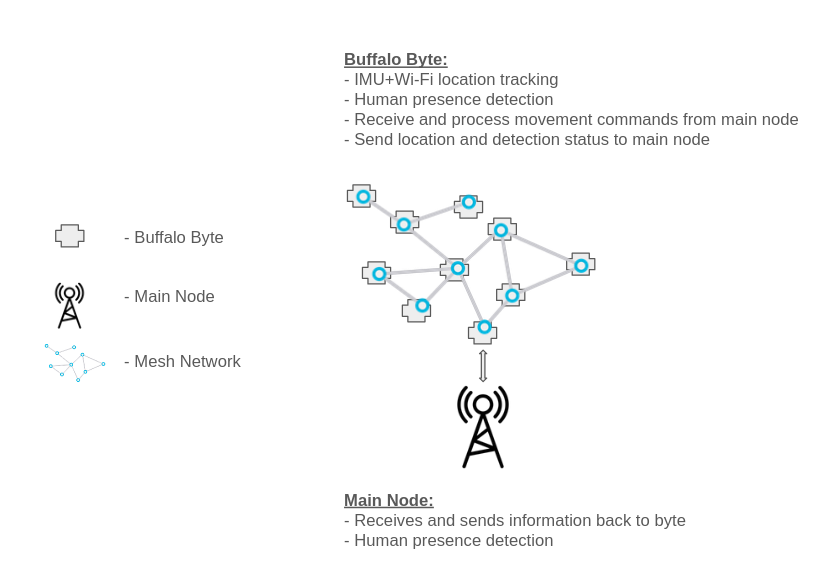
\includegraphics[scale=0.4]{conceptual-model}\\
\end{center}
Our design will be composed of three main sub-systems, the Buffalo Byte, the mesh network, and the main node. We have given a general outline of each subsystem below.
\begin{enumerate}
	\item\underline{Mesh network}\\
	To create a mesh network, we will take advantage of the station+softAP Wi-Fi mode supported by the ESP8266, along with the ESP-WIFI-MESH software library provided by Espressif. Each Buffalo Byte in the mesh network will act as both a host and a router, allowing them to forward packets not intended for them down the mesh network to the intended host. As long as all Buffalo Bytes are within range of eachother, data will be able to be sent to/from each Byte and to/from the main node, with each node in the network having its own IP address.

	\item\underline{Buffalo Byte}\\
	The Buffalo Byte will be responsible for three main tasks. Firstly, through the use of EKF aided IMU location tracking, it will be able to find its way to a specific set of coordinates while keeping track of its current location. The coordinates which the Buffalo Byte is to go to will be sent to it from the main node through the mesh network. The next task for which it will be responsible for will be to take one or more readings from a sensor. We are currently comparing options such as an active/passive infrared sensor, a thermal imaging sensor, or a combination of multiple sensors. These readings should be able to detect human presence (e.g. someone in the Bytes FOV trapped under rubble, unconcious on the ground, etc.) to some degree of certainty. This system is not meant to replace a human search team, but to instead provide information quickly as to where people may be concentrated, as well as locating the more readily apparent instances, so the sensor readings do not need to have absolute accuracy. The Buffalo Bytes last task will be to relay its location and the results of its most recent sensor reading back to the main node through the mesh network. Upon completion of these three tasks, it will await another movement instruction from the main node and repeat the cycle.

	\item\underline{Main node}\\
	The main node will be a server which could be hosted on any computer with Wi-Fi support and sufficient resources, in our case a Raspberry Pi 4. Whenever a Buffalo Byte stops to take a sensor reading, the server will receive a TCP packet containing a single-bit flag indicating whether or not human presence is suspected as well as the Buffalo Bytes current coordinates. Based on this information, the current coordinates of the other Buffalo Bytes in the mesh network, and the coordinates at which sensor readings have already been taken, the main node will send back a TCP packet to the Buffalo Byte containing the next set of coordinates at which it should take a sensor reading. The main node will choose this location such that the Buffalo Byte remains in range of the mesh network. The server will output to a webserver a list of the coordinates where a sensor reading suggesting human presence was taken.
\end{enumerate}

\section*{Measure of Success}
\subsection*{Technical Standards}
\underline{ISO 13482:2014}\\[0.25\baselineskip]
This standard describes the safety requirements for non-medical and non-industrial human aid robots, and the factors that must be satisfied in order for the robot to be considered safe for human interaction.\\[0.1in]
\underline{IEEE 42010}\\[0.25\baselineskip]
This standards describes best practice for organizing software-heavy systems in a modular manner. This will be relevant to our project because many of our subsystems are heavily software reliant. Building them in a modular way will make testing each individual components much easier as it allows for each subsystem to be tested completely isolated from the others.
\subsection*{Measurement Criteria}
\underline{Mesh Network}: Measure the average latency and packet loss when sending data over the mesh network.\\[0.5\baselineskip]
\underline{Location Tracking}: Measure the average offset between the predicted and measured location.\\[0.5\baselineskip]
\underline{Human Sensing}: Measure success rates for human detection and percentage of false positives.\\[0.5\baselineskip]
\underline{Pathfinding}: Create a list of obstacles and measure how reliably a Byte can navigate around them.
\subsection*{Measurement Plan}
When comparing possible approaches to designing a subsystem (e.g. sensor type, pathfinding algorithm, etc.), we will use the above measurement criteria to evaluate the alternatives and choose the most performant. Upon the completion of a subsystem, it will be tested by the appropriate criteria to establish a baseline measurement. As these subsystems are tweaked, we will test again to ensure that the changes result in better performance with respect to these criteria. Before implementing a design, we will check with the relevant standards mentioned above to ensure that the design would adhere to them.

\section*{Timeline}
\subsection*{Bob's Timeline}
\begin{enumerate}
	\item Create a software simulation environment for Buffalo Byte which simulates movement and IMU data
	\item Set up the mesh network, and confirm communication is possible between Bytes and the main node
	\item Create protocol for choosing a new location and sending the Byte to it
	\item Create a pathfinding algorithm for the Buffalo Byte to find the locations given to it by the main node
	\item Create the server/client applications for the Byte and the main node
	\item Conduct testing on the Byte Swarm in a physical environment, and make adjustments accordingly
\end{enumerate}
\begin{ganttchart}[bar height=0.7,y unit title=2\baselineskip,y unit chart=0.2in,vgrid,hgrid]{1}{22}
	\gantttitlelist{4,...,14}{2}\\
    \ganttbar{1}{1}{3}\\
    \ganttbar{2}{4}{6}\\
    \ganttbar{3}{7}{8}\\
    \ganttbar{4}{9}{13}\\
    \ganttbar{5}{14}{16}\\
	\ganttbar{6}{17}{20}
\end{ganttchart}
\subsection*{Dylan's Timeline}
\begin{enumerate}
	\item Write equations and create a program to track position data using the IMU and EKF
	\item Create a program to enhance this movement tracking via Wi-Fi triangulation
	\item Create a pathfinding algorithm for the Buffalo Byte to find the locations given to it by the main node
	\item Finalize and implement protocols for server/Byte communication
	\item Conduct testing on the Byte Swarm in a physical environment, and make adjustments accordingly
\end{enumerate}
\begin{ganttchart}[bar height=0.7,y unit title=2\baselineskip,y unit chart=0.2in,vgrid,hgrid]{1}{22}
	\gantttitlelist{4,...,14}{2}\\
    \ganttbar{1}{1}{5}\\
    \ganttbar{2}{6}{9}\\
    \ganttbar{3}{10}{13}\\
    \ganttbar{4}{14}{16}\\
	\ganttbar{5}{17}{20}
\end{ganttchart}
\subsection*{Zhiyun's Timeline}
\begin{enumerate}
	\item Explore sensor options and test alternatives to choose the best option
	\item Interface the selected sensor with the ESP8266
	\item Create a pathfinding algorithm for the Buffalo Byte to find the locations given to it by the main node
	\item Finalize and implement protocols for server/Byte communication
	\item Conduct testing on the Byte Swarm in a physical environment, and make adjustments accordingly
\end{enumerate}
\begin{ganttchart}[bar height=0.7,y unit title=2\baselineskip,y unit chart=0.2in,vgrid,hgrid]{1}{22}
	\gantttitlelist{4,...,14}{2}\\
    \ganttbar{1}{1}{5}\\
    \ganttbar{2}{6}{9}\\
    \ganttbar{3}{10}{13}\\
    \ganttbar{4}{14}{16}\\
	\ganttbar{5}{17}{20}
\end{ganttchart}

\end{document}
